%!TEX root = mieic-en.tex

\chapter{Literature Review} \label{chap:sota}

\section*{}
\textit{
Neste capítulo é descrito o estado da arte e são
apresentados trabalhos relacionados para mostrar o que existe no
mesmo domínio e quais os problemas em aberto.
Deve deixar claro que existe uma oportunidade de desenvolvimento que
cobre alguma falha concreta .
O capítulo deve também efetuar uma revisão tecnológica às principais
ferramentas utilizáveis no âmbito do projeto, justificando futuras
escolhas.
}

Resenha utilizaçao computer vision em trafego e em transportes
Concluir com os desafios da armis (drive, quere aplicaro computer vision para automatizar determinados aspetos)
Sequência de funcionalidades que respondem ao desafio da Armis(segmentaçao,deteçao,...)
Uma secção para cada um

Tese Gustavo Lira / Pedro Loureiro

\section{History of Computer Vision}

Computer vision appeared as an area of investigation around the mid 60's at the MIT by Professor Larry Roberts, whose PhD. thesis focused on methods to extract 3D information from a 2D image ~\cite{huang_computer_1996} in order to reconstruct entire scenes from the geometry gathered. This area is now considered by the ACM as a branch of artificial intelligence according to the 2012 ACM Computing Classification System ~\cite{acm_2012_2012}. From this point onward scientists began applying the techniques developed in multiple fields.

The use of computer vision in manufacturing industry was among the first to be explored, as there were already multiple robots working in the assembly lines of the factories that needed to be improved, as noted by Stout in 1980 ~\cite{stout_computer_1980}. These robots were becoming outdated due to the lack of interaction with the environment. This meant that for a robot to work with a part in an assembly line it needed to be placed in a pre-determined position, and any deviation could mean that the line needed to be stopped. Michael Baird relates in ~\cite{l._baird_sight-i:_1978} a computer vision system developed to inspect circuit chips rotation deviation in a welding base, indicating to the welder that the chip needed to be adjusted. Computer vision was also used as a tool to automatically analyse weather satellite images ~\cite{binford_computer_1973-2} and multidimensional medical images ~\cite{ayache_medical_1998}, with applications being developed in these areas being now common in our daily life.

\subsection{Computer Vision in Intelligent Transport Systems}

Regarding intelligent transport systems (ITSs), the use of computer vision to aid in the analysis of traffic has been increasing in the last years due to the decreasing costs of hardware, both cameras, storage and processing power, as well as the growing knowledge to extract useful data from the video gathered. In contrast to the high installation and upkeep costs of other traffic control tools such as Inductive Loop Detectors and Microwave Vehicle Detectors, applying computer vision to handle these tasks is a profitable option for entities in charge of the analysis of this data.

One of the first works applying computer vision to analyse traffic was published in 1984 ~\cite{dickinson_image_1984} and detected and measured movement in a sequence of frames. Since then, multiple fields of study have been created, not only for the measuring of traffic, as explored in ~\cite{lira_computer-vision_2016}, ~\cite{buch_review_2011-1} and ~\cite{hashmi_analysis_2012} where the authors evaluate methods to analyse traffic in urban environments, but also for the analysis of the environment around a self-driven vehicle, reading traffic signs using multiple approaches using convolutional neural networks ~\cite{soendoro_traffic_2011} or using bag-of-visual-words ~\cite{supriyanto_unsupervised_2016}, or to automatize the parking process as discussed in ~\cite{hammoudi_self-driven_2016}. Recently some studies have surfaced where the authors discuss the analysis of passenger numbers and behaviour inside vehicles, in order to enforce traffic laws ~\cite{loce_detection_2017-1}.

For our application however we need to focus on the aspect of traffic analysis, and in order to understand what traffic analysis software needs to accomplish, it is convenient to study what composes a typical traffic scene. Usually the scenes are viewed from a top-down perspective that places the cars against the road as background, as seen in ~\ref{fig:hh_traffic}. The vehicles have a roughly regular rectangular shape when viewed from the top, with little variation when the camera is rotated, however their textures vary heavily, making it difficult for a detector to work based on the vehicles image representation ~\cite{badenas_applying_1998}. However, depending on the camera position there can be object occlusion by other objects or scene components, which makes it difficult to detect and track vehicles relying solely on subtraction based segmentation techniques.

\begin{figure}[h]
  \begin{center}
    \leavevmode
    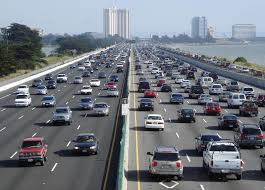
\includegraphics[width=0.5\textwidth]{traffic_scene}
    \caption{Typical High-Way Traffic Scene}
    \label{fig:hh_traffic}
  \end{center}
\end{figure}

The scenes also have varying light according to the time of the day, and proposed solutions need to adapt to these changes as fast as possible, otherwise data might be lost. Other weather conditions can also interfere with the analysis, such as fog and rain, and need to be addressed when designing solutions.

\subsection{Our Challenge}

The "Analytics Server" module of the "Video Server" project had a list of requirements that needed to be \todo{Acabar}

Detetar eventos relevantes
	Contra mao
	Objetos caidos

Contar Veiculos

Apenas para camaras fixas


\section{Foreground Segmentation}

Image segmentation is the process through which  an image is separated into its different regions according to the desired output, usually objects of interest. These regions are composed by pixels that have a common characteristic ~\cite{shapiro_computer_2001} dependant on the desired result. There are several ways one can accomplish an adequate segmentation of an image, and the most relevant ones to our purpose are described below.

\subsection{Background Subtraction}

Background Subtraction is a segmentation technique based on the analysis of the difference of consecutive frames and use that information to create a background model, a representation of what the image looks like without any moving objects present. Given the nature of the process, cameras must be static and although some research has been made to overcome this issue ~\cite{li_detection_2012} ~\cite{sheikh_background_2009} ~\cite{zamalieva_background_2014}, this is beyond the scope of the project, due to the requirements given.

There are however a number of different ways to implement the background subtraction developed across the years with increasing segmentation accuracy and computational performance. Piccardi presented an overview of the most relevant ones in ~\cite{piccardi_background_2004}, aiming to present each method's strengths and weaknesses. From this work we can present a list of the algorithms considered for implementation in the project.

\subsubsection{Frame Differencing}

This is the simplest approach to the problem as it only considers two frames at a time, making it only work in certain scenarios where the speed of the objects and frame rate of the camera allow it. In this model a pixel is considered as foreground if it satisfies the equation presented in ~\ref{eq:frame_diff}, and since the only parametrizable value is the Threshold, the whole segmentation process is very sensitive to any changes in this value.

\begin{eqnarray}
\label{eq:frame_diff}
\left | frame_{i} - frame_{i-1} \right | >= Threshold
\end{eqnarray}
\subsubsection{History Based Background Model}

In order to make this segmentation method more robust, in the early 2000's Velastin ~\cite{lo_automatic_2001} and Cucchiara ~\cite{cucchiara_detecting_2003} proposed a mathematical model to take into consideration past frames when calculating the Background Model of the scene. The most simple version of the improved algorithm used a running average of the past frames as seen in ~\ref{eq:running_average}. This eliminates the need to store the frames in memory as the new average can be calculated using the previous results.

\begin{eqnarray}
\label{eq:running_average}
BackgroundModel _{i+1} = \alpha * Frame_{i} + (1-\alpha)* BackgroundModel _{i}
\end{eqnarray}

Instead of the running average one can use the median value of the last n frames, improving the method reaction to outlying values. In both however, the history can be just the n frames or a weighted average where recent frames have more weight. Both these methods cannot cope with intermittent changes on the background, such as moving leaves against a building facade, and to solve this problem a new approach was proposed, the Mixture of Gaussians which models each pixel according to a mixture of Gaussian distributions, usually 3 to 5, but in later research ~\cite{zivkovic_improved_2004} a method was developed to calculate the number of distributions needed on a per pixel basis.

\subsection{Object Based}

Object Based segmentation relies on the a priori knowledge of the geometry of the objects we want to extract from the image. It is mainly used in medical applications such as in ~\cite{snell_model-based_1993} where it is used to extract a model of the brain surface from MRI scans \todo{Acabar}

\section{Image Treatment}

This section will review some of the proposed methods to improve image quality before or during processing by removing noise, extracting unwanted features or enhancing relevant features for the processes involved.

\subsection{Blur}

In order to blur an image one needs to convolve it using a special kind of filter. The process of convolution in image processing consists in the application of a filter to every pixel of an image, returning a new image where each pixel is the result of the function to the pixel in the same position in the previous image. As we can see in ~\ref{fig:convolution} the application of a 3*3 mask, where all 9 values have the value 1/9, results in a image where each pixel value equals the mean of itself and surrounding neighbours in the original image.

\begin{figure}[h]
  \begin{center}
    \leavevmode
    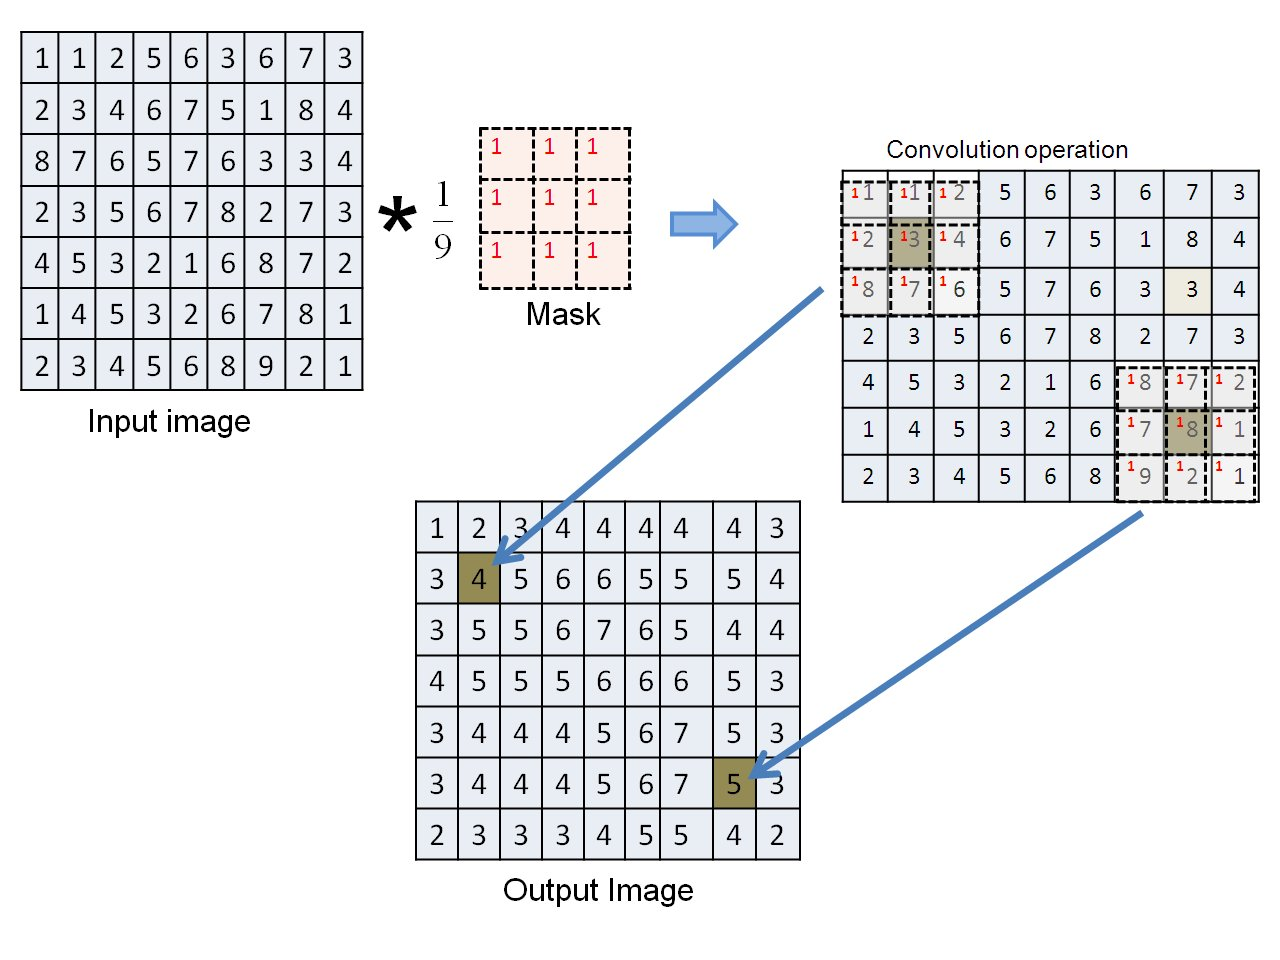
\includegraphics[width=0.7\textwidth]{convolution}
    \caption{Convolution Example ~\cite{labs_theory_2017}}
    \label{fig:convolution}
  \end{center}
\end{figure}

While this is the simplest blur processing we can apply to an image, there are more complex ones that yield better results. The one most often used in image processing is the Gaussian Blur, which uses a square filter with values calculated with the equation in ~\ref{eq:gaussian} from ~\cite{shapiro_computer_2001}.

\begin{eqnarray}
\label{eq:gaussian}
G(x,y) = \frac{1}{2\pi \sigma ^{2}}e^{-\frac{x^{2}+y^{2}}{2\sigma ^{2}}}
\end{eqnarray}

This equation returns a filter consisting of concentric circles that results in a smooth blurring of the images due to the application of the same power of blurring from equidistant pixels. The function can be tuned to the needs of the process through the $\sigma$ value, returning a sharper or softer blur filter as seen in figure ~\ref{fig:gaussian}.

\begin{figure}[h]
  \begin{center}
    \leavevmode
    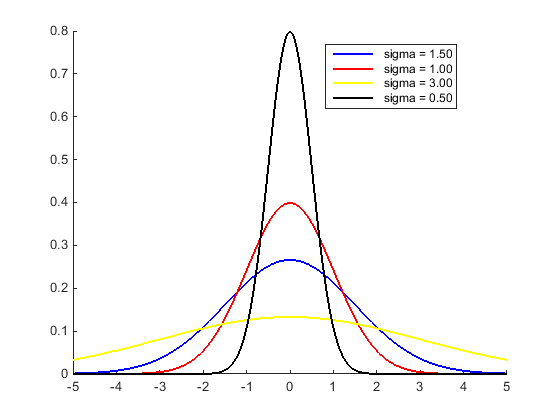
\includegraphics[width=0.5\textwidth]{gaussian}
    \caption{Gaussian Function Variation with Sigma Value}
    \label{fig:gaussian}
  \end{center}
\end{figure}

This kind of filters have multiple uses in computer vision. Blurring an image removes the grain noise it contains, creating more even surfaces that ease the process of image processing, as well as making edges easier to detect with edge detection algorithms.

\subsection{Edge Detection}

Detecting the edges in an image is an important step into the understanding of its contents, allowing segmentation based on surfaces and a spatial perception of the scene. The work presented by Marr and Hildreth ~\cite{Marr1980TheoryOE} defines edges as part visual and part physical and proceeds to show that the two are interconnected. The first step of the proposed process is to calculate the zero-crossings of equation ~\ref{eq:intensity}, the Laplacian of a two dimensional Gaussian applied to different scales of the image, which returns both the points of intensity change and the slopes of the function at that point.

\begin{eqnarray}
\label{eq:intensity}
\nabla^{2} G(x,y)*I(x,y)
\end{eqnarray}

What the authors noted was that if an edge was detected at a certain scale it appears also at adjacent scales, which they called "spatial coincidence assumption". This theory can be reversed, if there is a convergence of edges on multiple scales there is a real physical edge, and based on this, if we find zero-crossings on neighbour scales, we can assume there is a real edge in that region. From here multiple implementations of the algorithm appeared, the most used one being presented below, the Canny Edge Detector using a Sobel filter. Although this was among the first implementations of an edge detector it is the most rigorously defined one and is still considered to be state of the art.

The Sobel filter is used to create an image that accentuates the edges of an original image. This process works by convolving two kernels with the image, one for the horizontal and the other for the vertical direction, that return the intesity change in that pixel for each one. The filters can be seen in ~\ref{eq:sobel_filter} as they were presented by Irwin Sobel ~\cite{sobel_isotropic_1989}.

\begin{eqnarray}
\label{eq:sobel_filter}
G_{x} =
\begin{bmatrix}
+1 & 0 & -1\\ 
+2 & 0 & -2\\ 
+1 & 0 & -1
\end{bmatrix} , G_{y} = \begin{bmatrix}
+1 & +2 & +1\\ 
0 & 0 & 0\\ 
-1 & -2 & -1
\end{bmatrix}
\end{eqnarray}

Using $G_{x}$ and $G_{y}$ it is possible to retrieve the regions of the image that contain edges by calculating the magnitude of the gradient vector as the square root of the sum of the squares of both components and thresholding these values. One of the features of this process is the ability to retrieve the direction of the edge from these values, using the inverse tangent operation.

The Canny Edge Detector uses the result of the Sobel filter as input and filters the most relevant edges as well as thinning them to 1-pixel wide lines. To accomplish this Canny used an optimization process comparing the value of the gradient magnitude to the one of the neighbour pixels along the direction returned by the Sobel filter, and keeping only the one with the largest value along the edge.

\subsection{Mathematical Morphology}

Mathematical Morphology is a set theory, offering solutions to multiple image processing problems, where the sets are composed of tuples corresponding to the 2D coordinates of each pixel in the image. These sets identify the white or the black pixels in a binary image, depending on the convention adopted, or the intensity of the pixel in a grey-scale image ~\cite{dougherty_introduction_1992}. During this chapter we will consider that all images are binary and that the pixels to process are black in a white background. This theory provides a set of operators that can be used to detect convexity and connectivity of shapes in an image, enhancing features, detecting edges and removing noise. 

The operators are defined by a structuring element, also known as kernel, a set of coordinates represented in a binary image, usually much smaller than the image to process. The centre of the kernel is not in the top left corner as in most images but rather in the geometrical centre, meaning that there some of the pixels have negative coordinates. The kernel shapes in figure ~\ref{fig:morh_operators} are the ones typically used for most applications, but the process allows the user to design their own if needed.

\begin{figure}[h]
  \begin{center}
    \leavevmode
    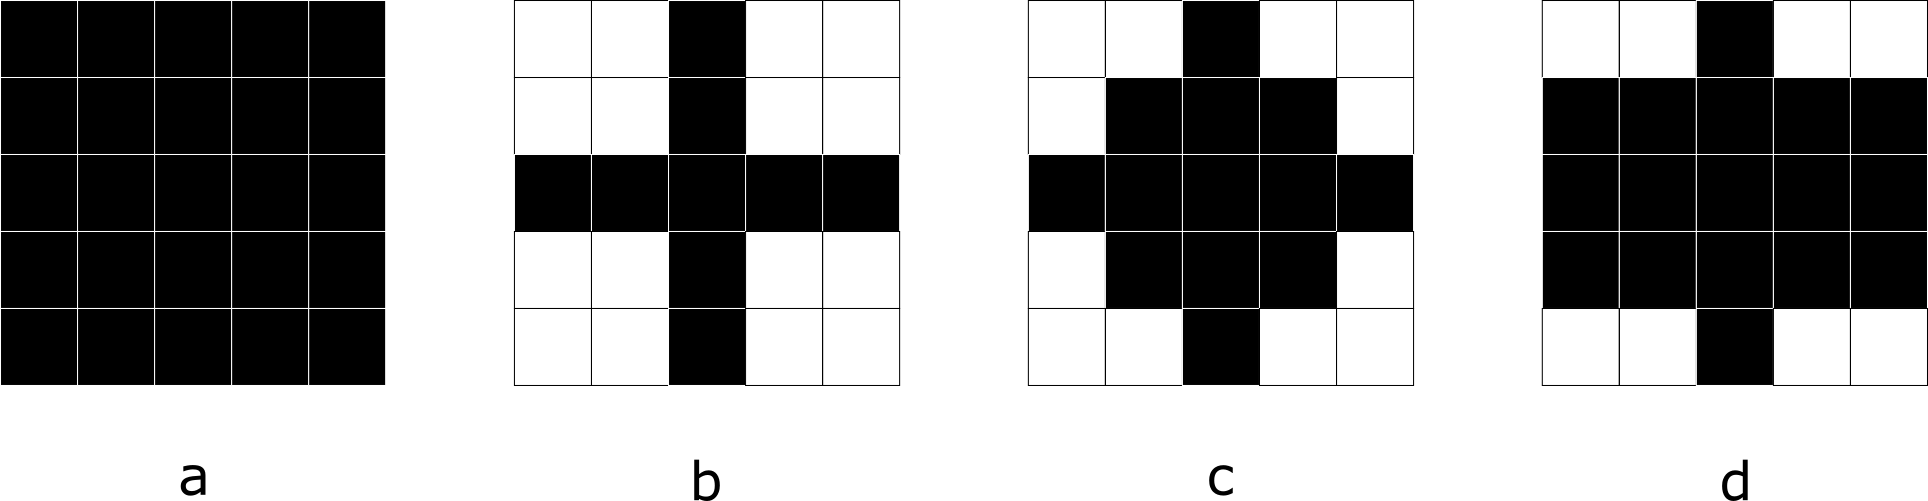
\includegraphics[width=0.9\textwidth]{morph_operators}
    \captionsetup{justification=centering}
    \caption{Morphology Operators typical structuring elements (5x5)\\a) Rectangular b) Cross c) Diamond d) Elliptical}
    \label{fig:morh_operators}
  \end{center}
\end{figure}

According to Gonzalez and Woods ~\cite{gonzalez_digital_1992} an operator is defined by an image and a structuring element, and to run it the origin point of the element needs to be placed at every pixel of the image. At each of these locations a verification is done depending on the operation being performed and an output image is created using the independent output of these operations.

The two most basic operations are erosion and dilation, essential to morphological processing. The erosion operator translates the structuring element to every black pixel of the image and in each position checks if all the active pixels of the kernel match with black pixels in the image. If it is true then the returned pixel is black, otherwise it is white. An example of the usage of such an operator can be seen in figure ~\ref{fig:erosion}. These operators are mainly used to remove noise from binary images or to separate objects to enable individual labelling and counting.

\begin{figure}[h]
  \begin{center}
    \leavevmode
    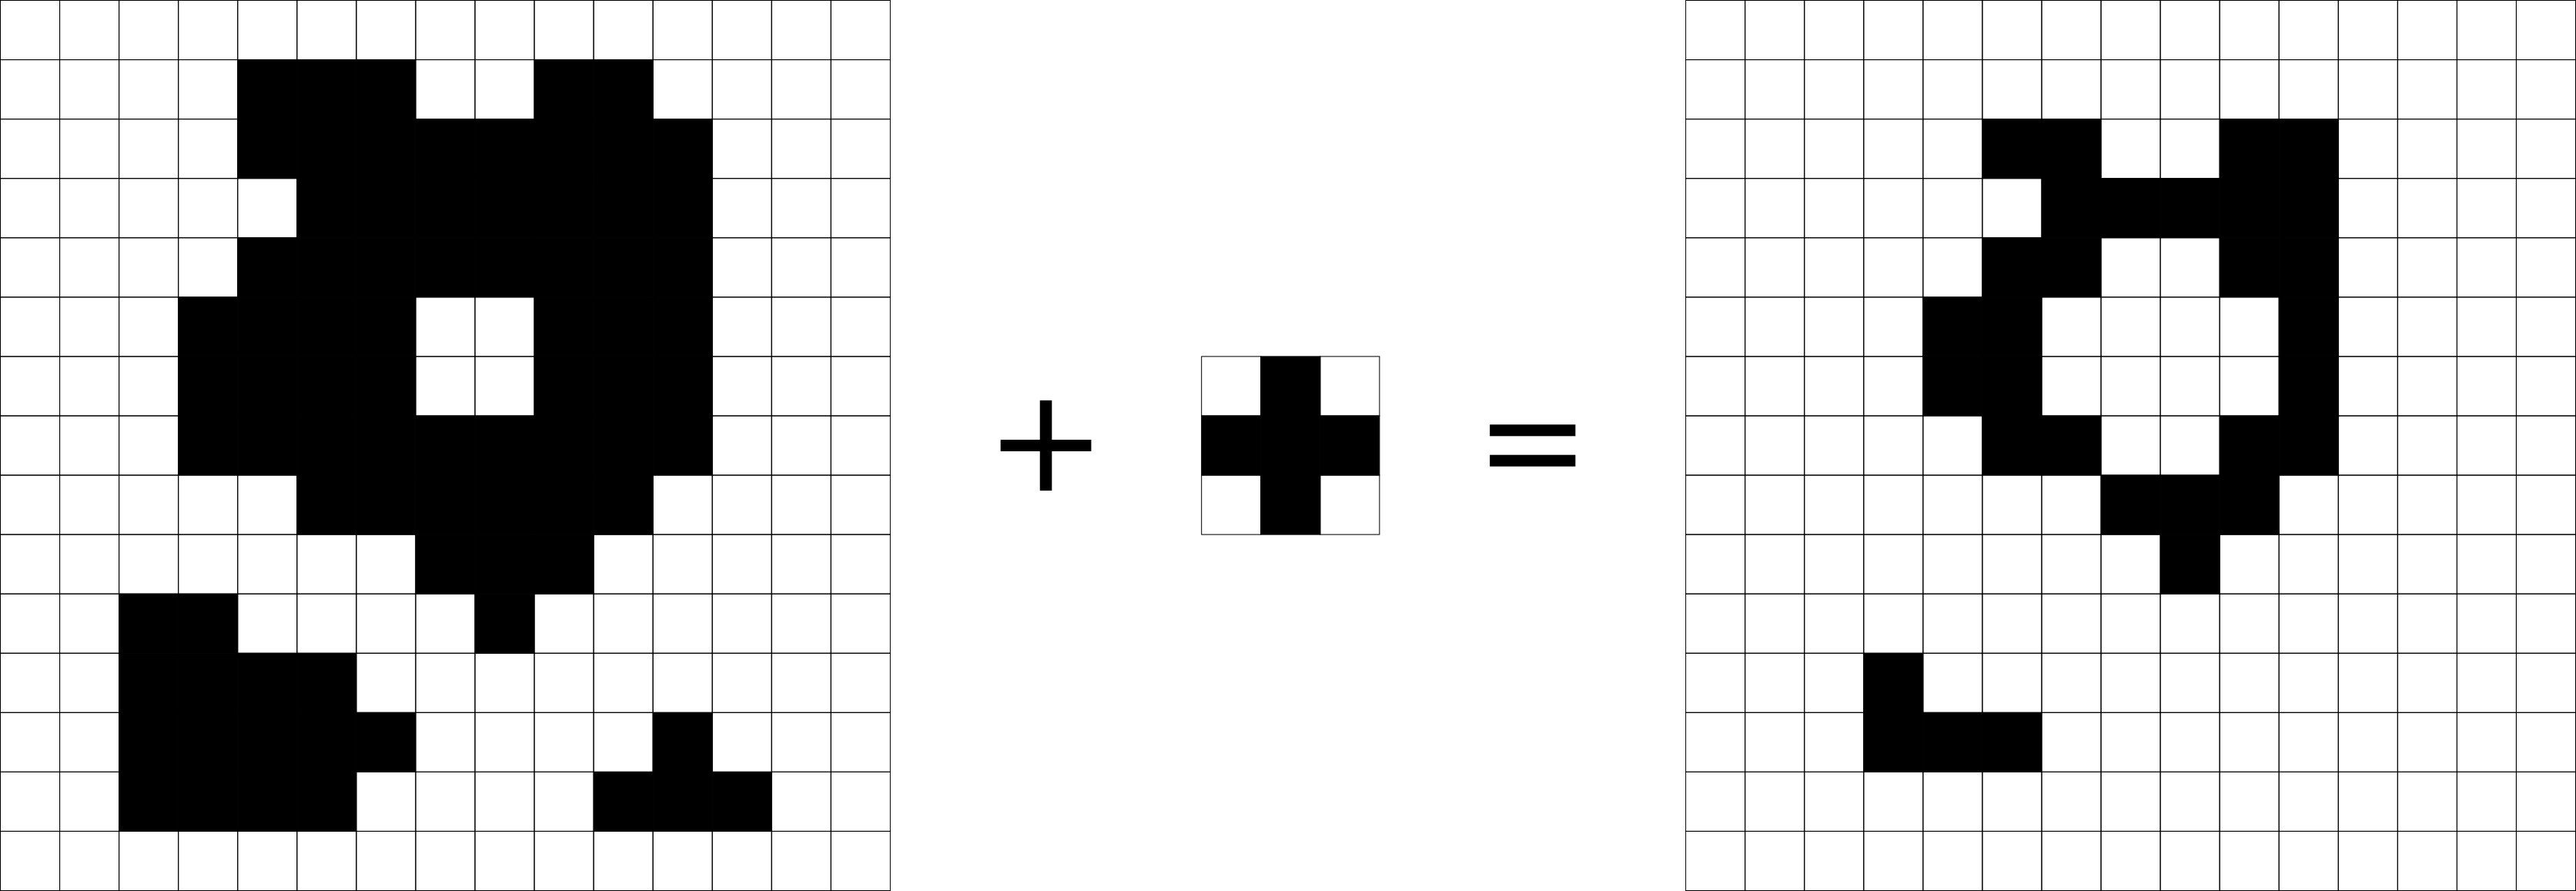
\includegraphics[width=0.9\textwidth]{erosion}
    \captionsetup{justification=centering}
    \caption{Result of the Erosion operator using a cross 3x3 kernel}
    \label{fig:erosion}
  \end{center}
\end{figure}

The dilation operator works by setting to black all the pixels that match the position of the translated kernel's pixels, resulting in the closing of holes in the image and the enhancing of small features. Results can be seen in figure ~\ref{fig:dilation}. Using a non-symmetrical kernel the dilation will be directional, enabling the user to fine tune the process to their needs.

\begin{figure}[h]
  \begin{center}
    \leavevmode
    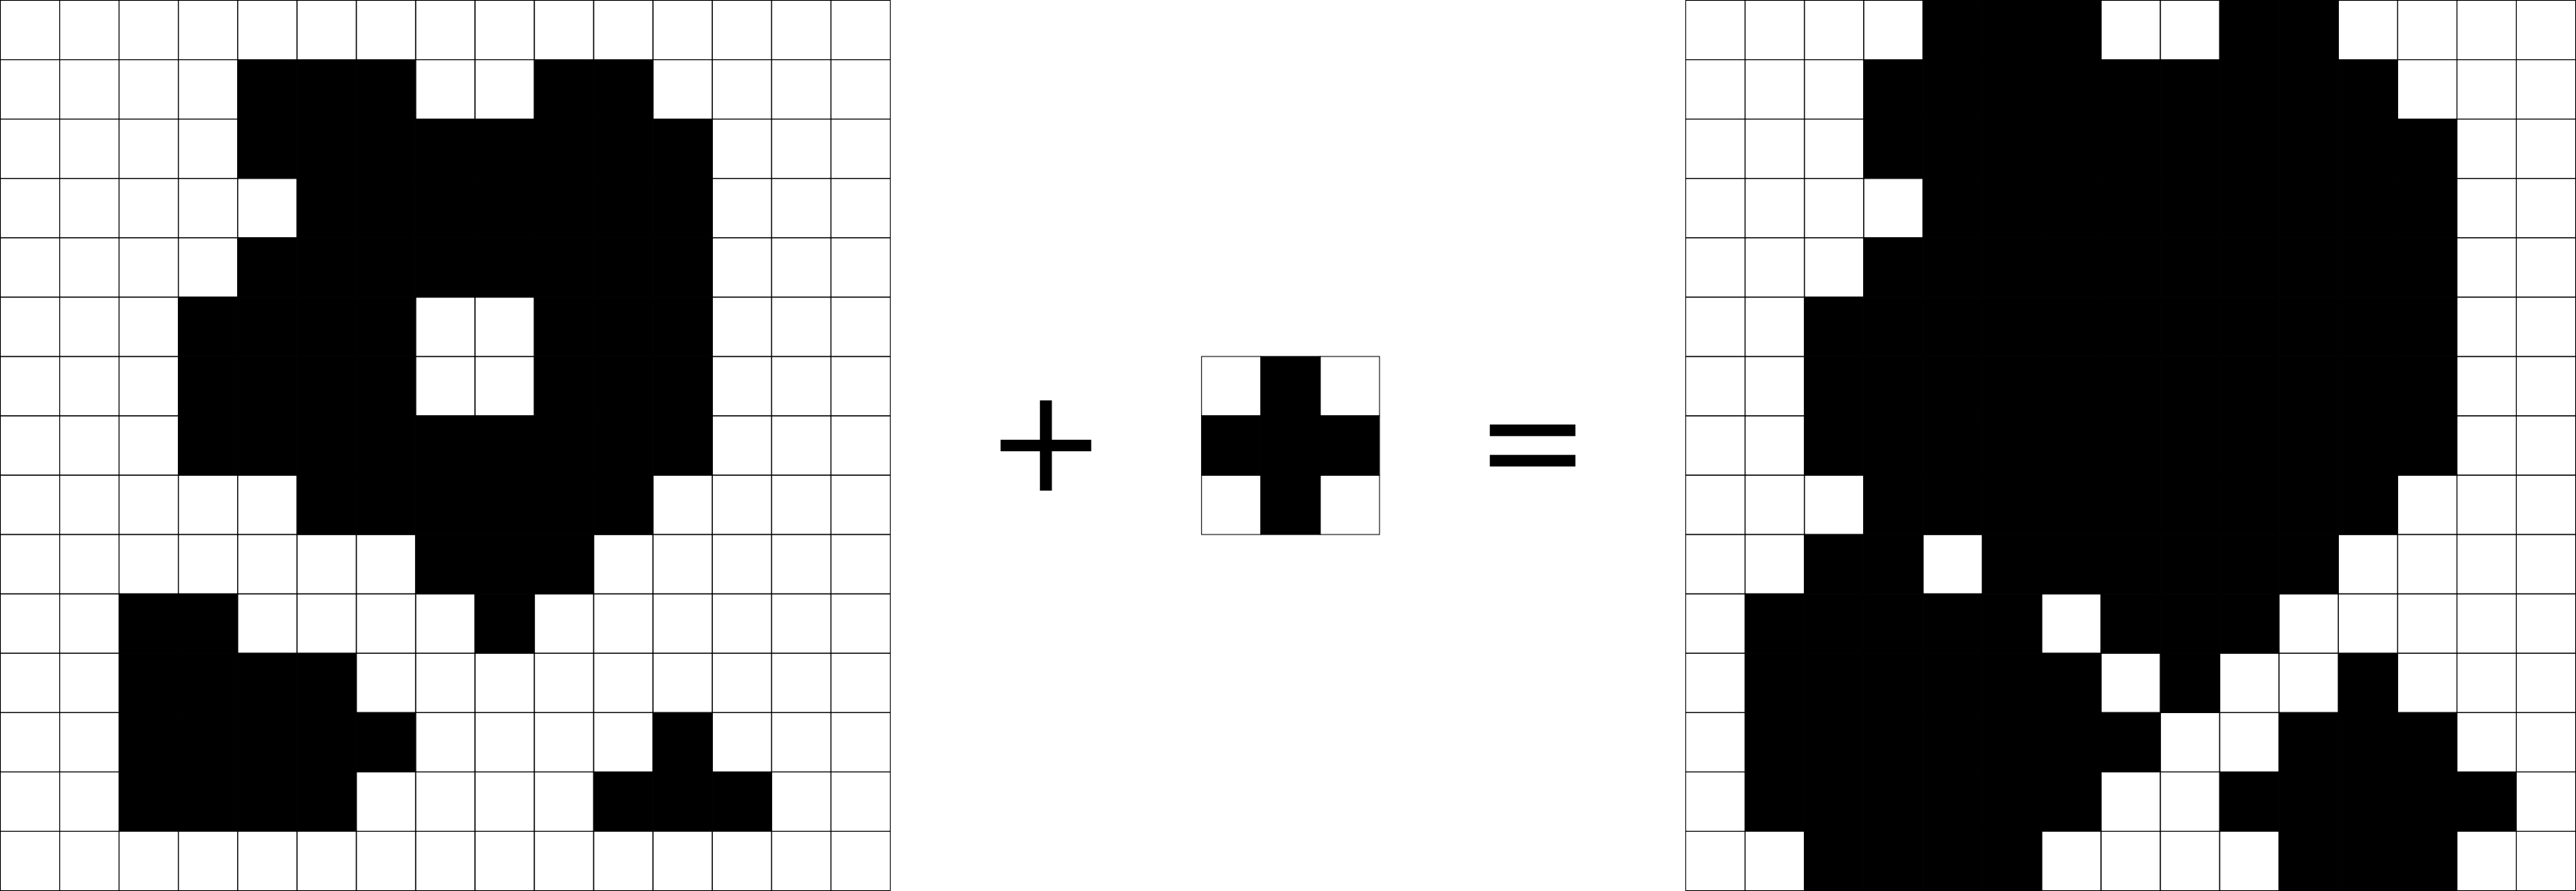
\includegraphics[width=0.9\textwidth]{dilation}
    \captionsetup{justification=centering}
    \caption{Result of the Dilation operator using a cross 3x3 kernel}
    \label{fig:dilation}
  \end{center}
\end{figure}

The dilation and erosion operators can be combined to form the opening and closing operators. An opening operator is formed by an erosion followed by a dilations using the same structuring element. This results in a less destructive erosion, preserving some of the image details as seen in figure ~\ref{fig:opening}. The closing operator is formed by a dilation followed by an erosion and the results can be seen in figure ~\ref{fig:closing}. It is commonly used to remove salt noise and to extract objects of a particular shape as long as they all share the same orientation ~\cite{fisher_morphology_2003}.

\begin{figure}[H]
  \begin{center}
    \leavevmode
    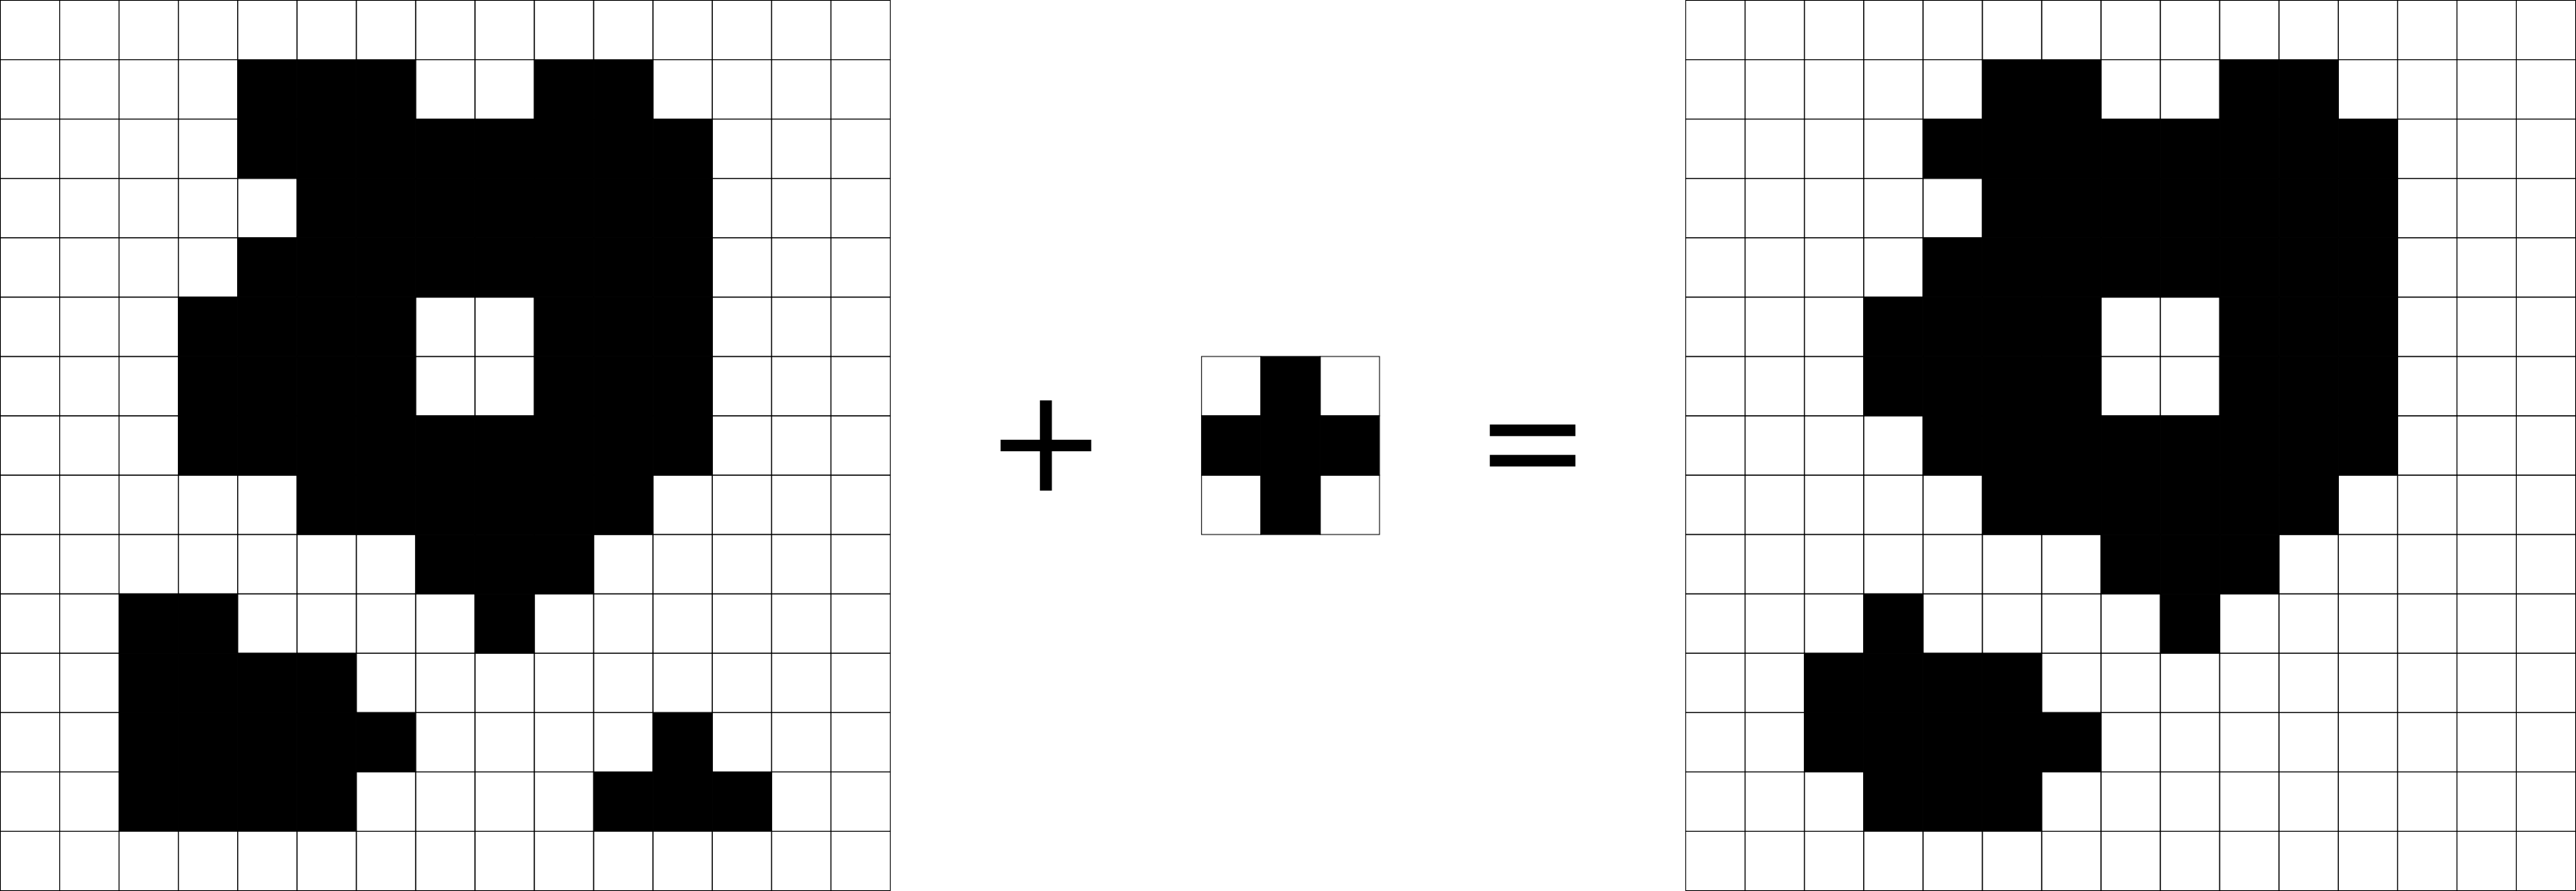
\includegraphics[width=0.9\textwidth]{opening}
    \captionsetup{justification=centering}
    \caption{Result of the Opening operator using a cross 3x3 kernel}
    \label{fig:opening}
  \end{center}
\end{figure}

\begin{figure}[H]
  \begin{center}
    \leavevmode
    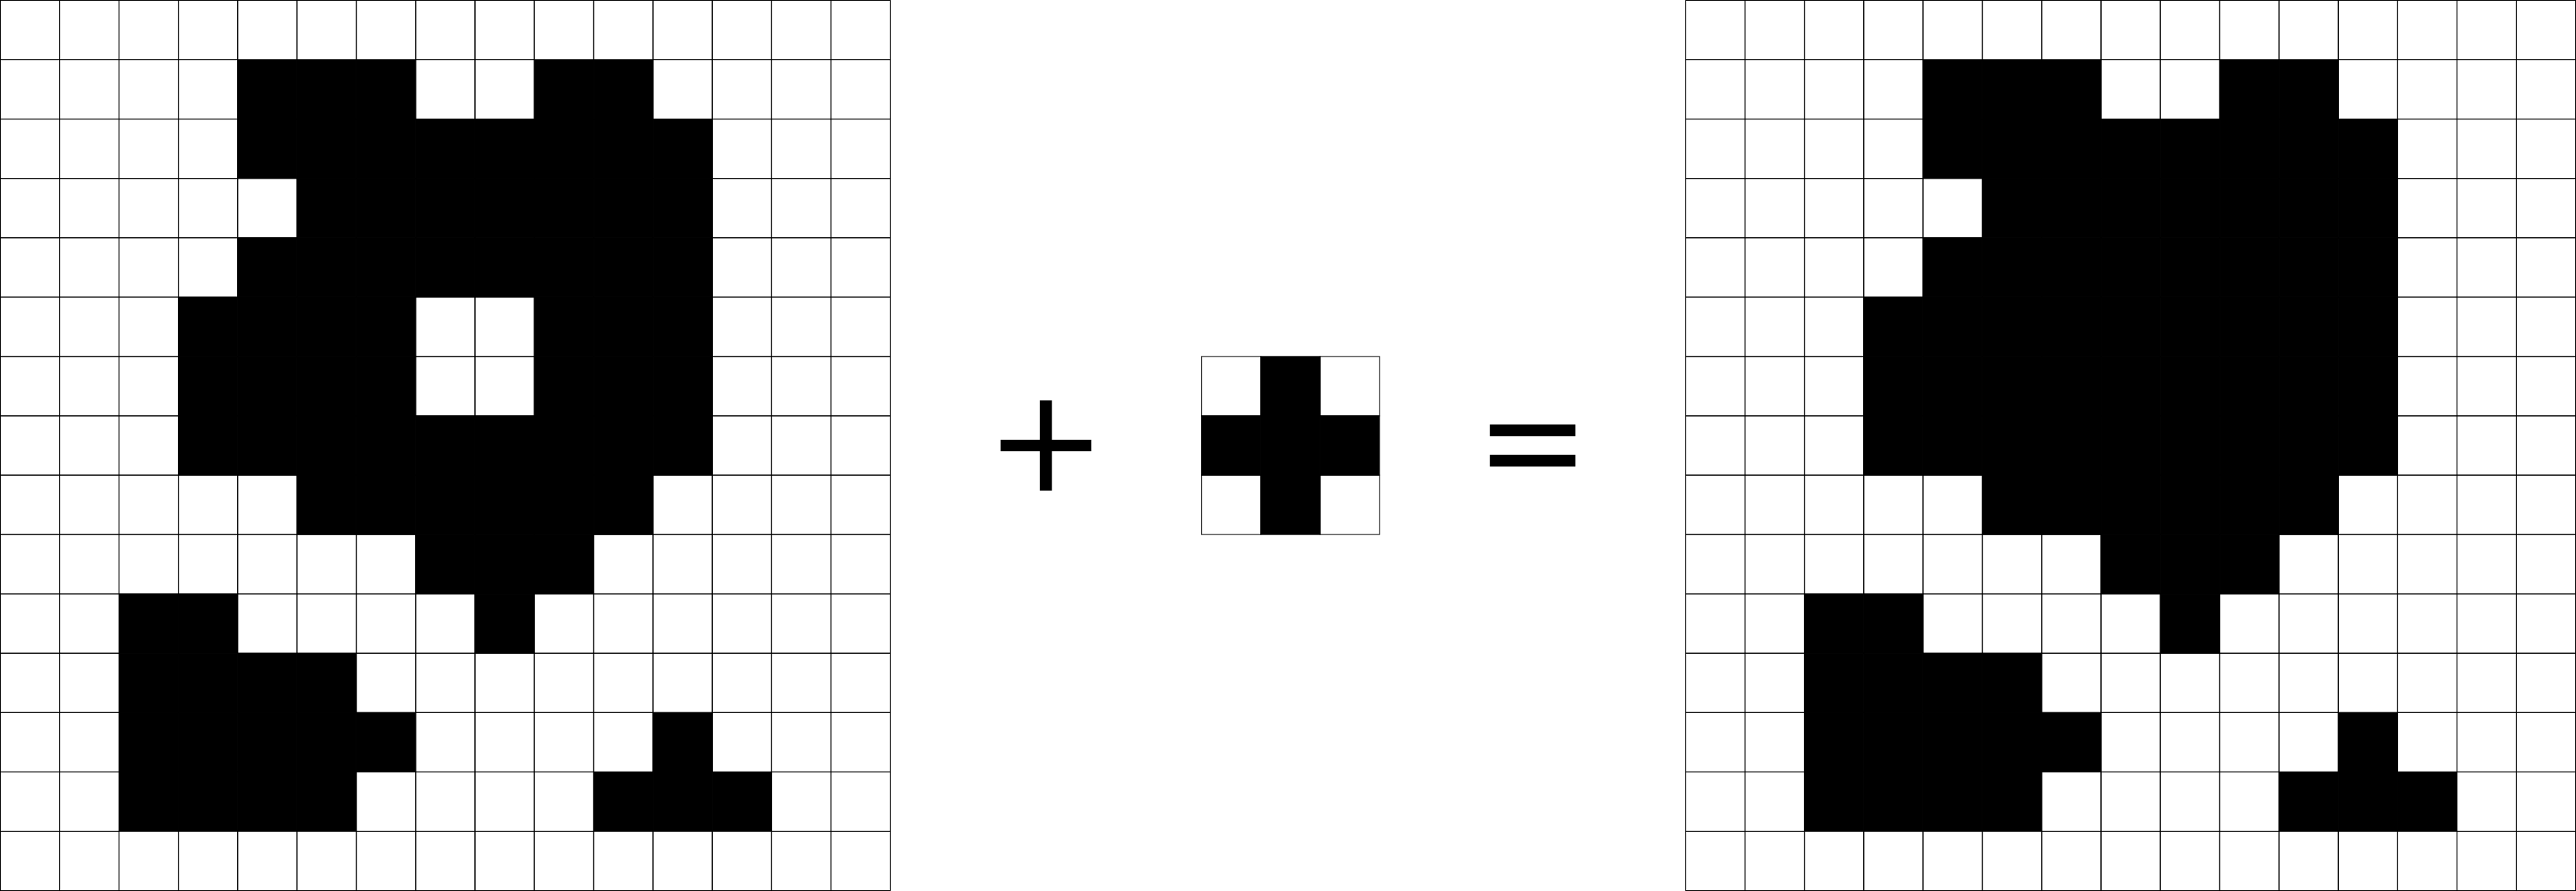
\includegraphics[width=0.9\textwidth]{closing}
    \captionsetup{justification=centering}
    \caption{Result of the Closing operator using a cross 3x3 kernel}
    \label{fig:closing}
  \end{center}
\end{figure}

\subsection{Shadow Removal}

Since shadows can be detected as foreground during the segmentation process, a process to remove them is important in certain scenarios. We will now describe some of the more interesting proposed methods to perform this task in this section.

In ~\cite{prati_shadow_2001} Prati et al. discussed how critical the shadow removal process is to traffic analysis, and they proceed to compare two ITS \todo{Adicionar a abreviaçoes} management systems, SAKBOT (Statistical and Knowledge-BasedObject Tracker) and ATON(Autonomous Transportation Agents for On-scene Networked incident manager), developed in Italy and the United States of America respectively.

SAKBOT adopts a method presented in ~\cite{cucchiara_statistic_2000}, which uses the chrominance information, converting pixel colours from RGB to HSV space, as it most closely relates to the human perception of colour. The process then evaluates how the scene colours components change due to the passing of vehicles and shadows, as seen in figure ~\ref{fig:sakbot-hsv}. From this we can extract that a shadow darkens a pixel and saturates its colour, and is the difference between an object point and a shadow point. The model then concludes that a point is considered as shadow if:

\begin{figure}[h]
  \begin{center}
    \leavevmode
    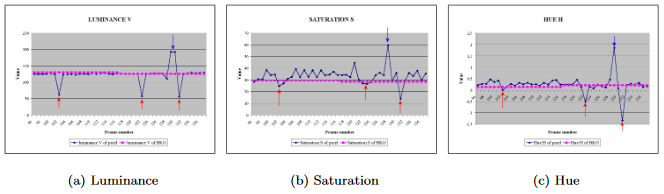
\includegraphics[width=0.9\textwidth]{sakbot-hsv}
    \captionsetup{justification=centering}
    \caption{HSV color space components change due to shadows. Red arrows indicate a shadow passing on the point. Blue arrow indicates a vehicle passing. ~\cite{prati_shadow_2001}}
    \label{fig:sakbot-hsv}
  \end{center}
\end{figure}

\begin{itemize}
	\item The ratio between the luminance of the image and the background is between two thresholds ($\alpha$ and $\beta$)
	\item The difference between the saturation of the image and the background is below a threshold ($\tau_{S}$)
	\item The absolute difference between the hue of the image and the background is below a threshold ($\tau_{H}$)
\end{itemize}

The $\beta$ value adjusts the tolerance to noise in the image to be considered as shadow and $\alpha$ takes into account the "power" of the shadow, how strong the light source is. $\tau_{S}$ and $\tau_{H}$ are considered by the authors to be harder to assign, and thus assigned empirically. This method main advantage is it's capability to detect moving shadows.

The method used by ATON is described in ~\cite{mikic_moving_2000} and begins by identifying three separate sources of information to detect shadows and objects:
\begin{itemize}
	\item Local information, the appearance of an individual pixel
	\item Spatial information, objects and shadows are compact regions
	\item Temporal information, the location of shadows and objects can be predicted from previous frames
\end{itemize}

The local information can be used to create a background model, both the mean and variance of the colour for each pixel when shadowed and not shadowed. In the segmentation process the values in the image are compared to the mean value of the background and if significantly different it is assigned a probability to belong to the background, foreground or shadow. The probability values are 0.3, 0.4 and 0.4 respectively. In the next iterations the neighbour pixels probabilities are considered in order to take advantage of the spatial transformation. The iterative process stops when there are no relevant changes, usually after the third iteration. Morphological operators are then computed over the output of the process to close unwanted openings in the regions. ATON does not use temporal information as of the time of the publication of the work. This process can identify with near 90\% accuracy shadows and object accuracy.

\todo{Se houver tempo adicionar mais metodos}

\section{Object Detection}

In this section we will analyse processes to detect objects of interest in images, a necessary step of any traffic surveillance system.


\subsection{Connected Component Labelling}

Connected component labelling is a process by witch the subsets of connected components are labelled according to the user needs. We will explore some of the most common implementations and how they evolved over time.

The one-pass solution presented by Abubaker ~\cite{abubaker_one_2007} is a fast and simple method to implement. It begins by labelling the first pixel of the image to 1, if it is a background pixel, skip to the next one, otherwise add it to a queue. While there are elements in the queue remove the one at the top and analyse its neighbours, if they are in the foreground add them to the queue with the current label. When there are no more elements in the queue increase the label number by one and proceed to the next unexplored pixel.

The two-pass solution presented by Shapiro et al. ~\cite{shapiro_computer_2001} uses the bi-dimensionality of the image data to transverse the pixels. The process, as the name implies, iterates over the image two times, the first time to assign temporary labels and the second to reassign these labels to the smallest ones available. It uses a neighbouring table to know what labels are adjacent to each other.

\begin{itemize}
	\item First pass
		\subitem Perform a Raster Scan to analyse all the pixels
		\subitem For each pixel, if it belongs to the foreground
			\subsubitem Get all its neighbours (four or eight depending on the connectivity assumed)
				\subsubitem Assign the smallest label from the neighbours
				\subsubitem Add the the previous and the new label to the neighbouring table
			\subsubitem If there are no neighbour pixels add a new label
	\item Second pass
		\subitem Perform a Raster Scan to analyse all the pixels
		\subitem For each pixel assign the lowest label from the neighbouring table
\end{itemize}

The process is illustrated in figure ~\ref{fig:two_pass_example}.


\begin{figure}[h]
  \begin{center}
    \leavevmode
    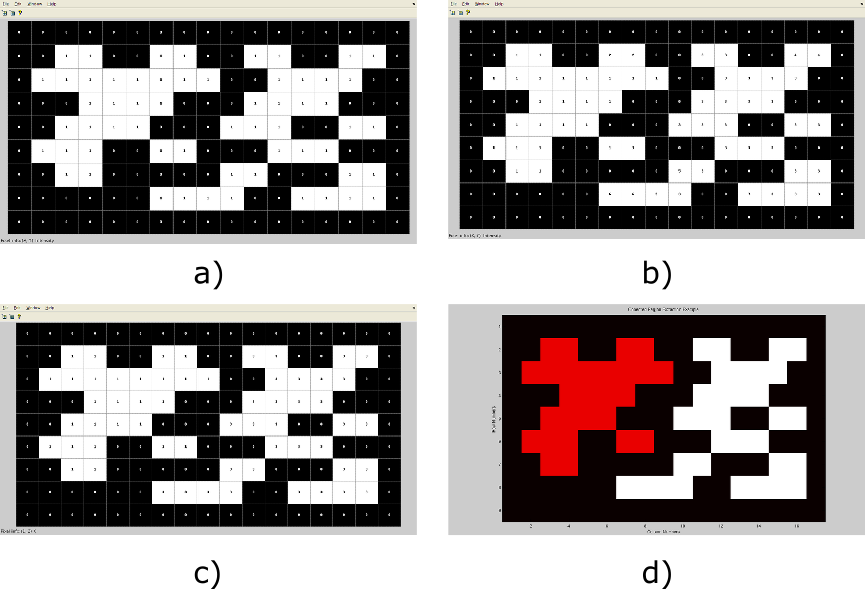
\includegraphics[width=0.9\textwidth]{two_pass_example}
    \captionsetup{justification=centering}
    \caption{Graphical example of the two-pass algorithm ~\cite{wikipedia_connected_2017}\\a) Original Image b) First Pass c) Second Pass d) Coloured Result}
    \label{fig:two_pass_example}
  \end{center}
\end{figure}

While these are the most basic solutions for the problem, a number of authors proposed enhancements to improve their performance, the most prominent ones being listed below:

\begin{itemize}
	\item Contour Tracing Labelling - F. Chang et al. ~\cite{chang_linear-time_2004} present a method that uses contour tracing to identify internal and external contours of each component. These contours are then used to label the connected components when the image is traversed horizontally by counting the number of contours passed.
	\item Hybrid Object Labelling - Herrero ~\cite{martin-herrero_hybrid_2007} presents a method that combines recursive and iterative analysis, finding unlabelled pixels and recursively finding their neighbours until a labelled one is found, then proceeding to the assignment in the adjacent rows.
	\item Improved Run-based Connected-component Labelling - L. He et al. ~\cite{he_run-based_2010}
\end{itemize}

\todo{Adicionar mais modelos?}

It is interesting to note the YACCLAB (Yet Another Connected Components Labelling Benchmark) ~\cite{grana_yacclab_2016} project, a benchmark platform that allows researchers to compare the performance of their connected components labelling methods to the methods of other researchers. The novelty of this platform is the fact that it uses the authors implementations instead of their own, allowing the algorithms to perform exactly as intended, with all the tweaks and tricks.

\subsection{Blob Detection}

A blob is defined as being a region with similar pixels based on some of their properties: intensity, 

\section{Object Tracking}



\section{Resumo ou Conclusões}

No final do capítulo deverá ser apresentado um resumo com as 
principais conclusões que se podem tirar. 

Vivamus non nunc nec risus tempor varius. Quisque bibendum mi at
dolor. Aliquam consectetuer condimentum risus. Aliquam luctus pulvinar
sem. Duis aliquam, urna et vulputate tristique, dui elit aliquet nibh,
vel dignissim magna turpis id sapien. Duis commodo sem id
quam. Phasellus dolor. Class aptent taciti sociosqu ad litora torquent
per conubia nostra, per inceptos himenaeos. 
